\documentclass[a4paper,11pt]{article}

% remove runningheads to submit
\usepackage[english]{babel}

% portuguese
\usepackage{graphicx}
\usepackage{float}
\usepackage{array}
\usepackage{listings}
\usepackage{courier}
\usepackage{color}
\usepackage{bnf}
\usepackage{appendix}
\usepackage[boxed,linesnumbered]{algorithm2e}

\lstset{
         basicstyle=\footnotesize\ttfamily, % Standardschrift
         %numbers=left,               % Ort der Zeilennummern
         numberstyle=\tiny,          % Stil der Zeilennummern
         %stepnumber=2,               % Abstand zwischen den Zeilennummern
         numbersep=5pt,              % Abstand der Nummern zum Text
         tabsize=3,                  % Groesse von Tabs
         %extendedchars=true,         %
         breaklines=true,            % Zeilen werden Umgebrochen
         keywordstyle=\color{red},
                %frame=b,         
 %        keywordstyle=[1]\textbf,    % Stil der Keywords
 %        keywordstyle=[2]\textbf,    %
 %        keywordstyle=[3]\textbf,    %
 %        keywordstyle=[4]\textbf,   \sqrt{\sqrt{}} %
         %stringstyle=\color{white}\ttfamily, % Farbe der String
         showspaces=false,           % Leerzeichen anzeigen ?
         showtabs=false,             % Tabs anzeigen ?
         xleftmargin=10pt,
         framexleftmargin=5pt,
         framexrightmargin=10pt,
         framexbottommargin=4pt,
         %backgroundcolor=\color{lightgray},
         %showstringspaces=false      % Leerzeichen in Strings anzeigen ?        
 }
 

\usepackage{caption}
\DeclareCaptionFont{blue}{\color{blue}} 
   \captionsetup[lstlisting]{singlelinecheck=false, labelfont={blue}, textfont={blue}}
   
 \DeclareCaptionFont{white}{\color{white}}
 \DeclareCaptionFormat{listing}{\colorbox[cmyk]{0.43, 0.35, 0.35,0.01}{\parbox{\textwidth}{\hspace{15pt}#1#2#3}}}
\captionsetup[lstlisting]{format=listing,labelfont=white,textfont=white, singlelinecheck=false, margin=-2pt, font={bf,footnotesize}}

% images: .png or .pdf w/ pdflatex; .eps w/ latex
\usepackage[latin1]{inputenc}

\usepackage[hyphens]{url}

% urls
%\usepackage{times}

% PS fonts
%\usepackage[T1]{fontenc}
\usepackage{a4wide}

%\hyphenation{}                  % explicit hyphenation
% entities
%\newcommand{\class}[1]{{\normalfont\slshape #1\/}}
\begin{document}
  \title{BioSeD - \textbf{Bio}logical \textbf{Se}quences \textbf{D}atabase\\\textbf{User Manual}}

  \date{\today}


  \maketitle


  \tableofcontents
  \listoffigures
  \listoftables
  \lstlistoflistings
  \clearpage

\section{Installation}

Before installing the application we will need to download the install package from the project
webpage. Two methods are available to download the application: downloading a release or
through Subversion, getting the most recent source code updates and fixes.

First, point your browser to \url{http://code.google.com/p/ibmc-bio-db/}.

If you want to use Subversion, select \textbf{Source} and once the page has loaded
you should see the Subversion checkout command. Run:

\begin{lstlisting}[language=c, frame=single]
$ svn checkout http://ibmc-bio-db.googlecode.com/svn/trunk/ biosed
\end{lstlisting}

If you want to download a stable release, select \textbf{Downloads} and click on the most up-to-date
version. Once the file as downloaded, run:

\begin{lstlisting}[language=c, frame=single]
$ tar zxvf biosed-version.tar.gz
\end{lstlisting}

For both methods, enter into the \textbf{biosed} directory. Take a look at the file \textbf{README}
and follow the instructions.

Once done, the application should be installed. Congratulations!

The install scripts creates one user for using the application, the \textit{admin} user, and, as name
says has more rights than \textit{normal} users.
Right now, you should point your browser to the application's location and login with this user.

Once the page has loaded, you should now see the main application's page.
On the left is the main menu, in the header there is a search box and at the main box is located
the main application's work area.

Right below the main menu there is a login box. Put \textit{admin} in the user field and
use the password you provided during the installation process.

\begin{figure}[H]
  \centering
    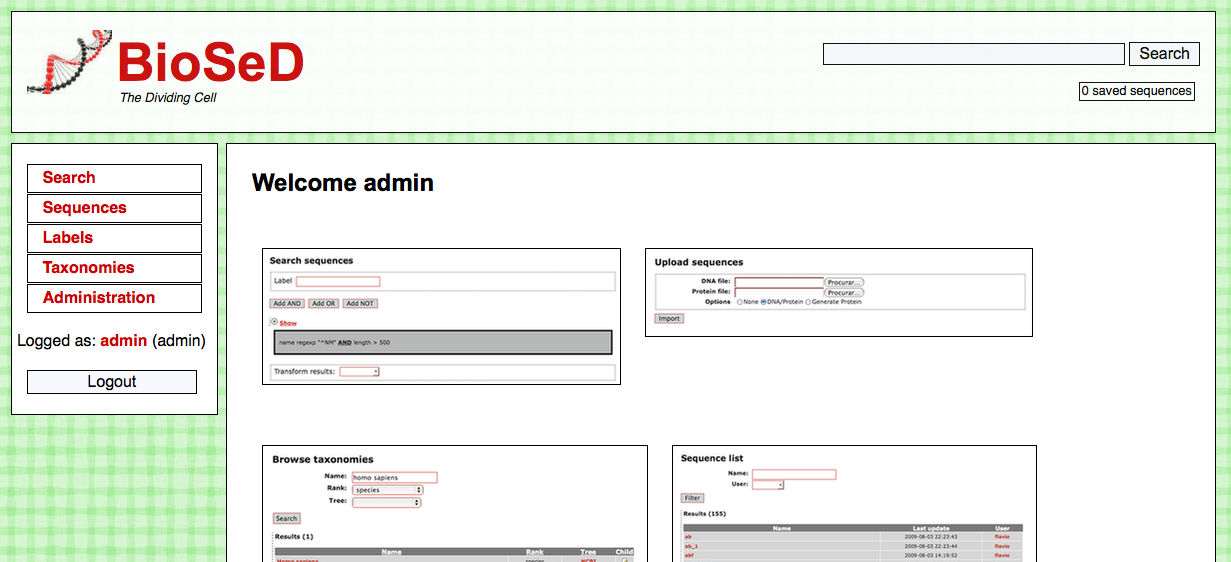
\includegraphics[scale=0.4]{interface.png}
  \caption{System home page.}
  \label{fig:home_page2}
\end{figure}

If you entered the correct password, the new page should look like Figure \ref{fig:home_page2}.

\section{Labels}

Label related options are found in the \textbf{Labels} submenu. For normal users
only the options \textbf{Labels - List} and \textbf{Labels - Export} are available.
The \textbf{admin} user has access to a few more options: \textbf{Labels - Add/New} and
\textbf{Labels - Import}.

\begin{figure}[H]
  \centering
    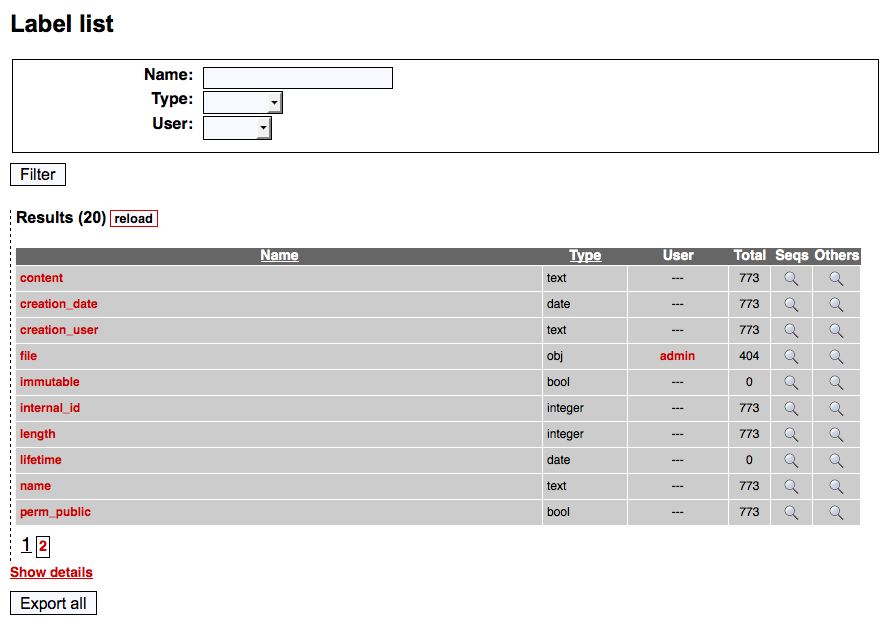
\includegraphics[scale=0.4]{label_list.png}
  \caption{Listing all labels}
  \label{fig:label_list}
\end{figure}

When listing labels, a page like Figure \ref{fig:label_list} should appear. The traditional
filter form is available and it is also possible to filter by label type.

The label types available are:
\begin{itemize}
  \item Integer: integer value.
  \item Float: float value.
  \item Text: text value.
  \item Position: pair of start and length values, representing a sequence's segment.
  \item Reference: pointer to another sequence.
  \item Taxonomy: pointer to a taxonomy.
  \item URL
  \item Bool: true/false value.
  \item Date: day, month and year triplet.
  \item Object: an uploaded file.
\end{itemize}

Still in this page, one can push the button \textbf{Export all} to export the current set of
labels being listed to XML. The button \textbf{Add new} redirects to the new label page, where one can
create a new label.

In the label list grid, special notes should be said about the columns:

\begin{itemize}
  \item Clicking on the label name redirects the application to the label's page.
  \item The column \textbf{Seqs} creates a new search page with sequences that contain that label.
  \item The column \textbf{Others} creates a new search page with sequences that do not contain that label.
\end{itemize}

\subsection{Creating new labels}

If you are an administrator, pushing the \textbf{Add new} button a new form will be presented.
The form contains all the fields needed to create a new label. They are:

\begin{itemize}
  \item \textbf{Name}: the label's name.
  \item \textbf{Type}: the label's type.
  \item \textbf{Code}: the code to generate a new label value using the sequence information as input.
  \item \textbf{Validation code}: code to validate a new label instance. Should return true if the value is valid, false otherwise.
  \item \textbf{Modification code}: block of code run after the sequence's content is updated. Should not return anything.
  \item \textbf{Comment}: comment about the label.
  \item \textbf{Must exist}: if true, every sequence must be annotated with this label, when that does not happen the label goes to the sequence's missing list.
  \item \textbf{Generate on creation}: if true when a sequence is created, the sequence will be automatically annotated with this label using the \textbf{Code} field.
  \item \textbf{Generate on modification}: if true and if the sequence is already annotated with this label, the label value is automatically changed using the \textbf{Code} field when the sequence's content is altered.
  \item \textbf{Deletable}: if true a specific label instance can be user deleted.
  \item \textbf{Editable}: if true a specific label instance can be user edited.
  \item \textbf{Default}: if true the label will me made system default and cannot be edited thereafter.
  \item \textbf{Public}: if true the label can be made part of public (no login) searches. 
\end{itemize}

All the code fields must be written in PHP \cite{php}.

Once created, you will be redirect to the label's page, where you can view or edit information about
the label. Each field can be changed by clicking on it.

Other options are present: \textbf{Delete} prompts you to delete the label, \textbf{Export} exports the label
to XML and \textbf{List labels} redirects you to the label list.

\subsection{Import / Export}

To export all labels you can use the option \textbf{Labels - Export} from the main menu. This
operation can be performed by any user.

Only the administrator is entitled to import files with labels. The option for this is
\textbf{Labels - Import}. There you should upload a XML file containing labels.
Once the file is processed a new report page is shown, as in Figure \ref{fig:import_labels}.

\begin{figure}[H]
  \centering
    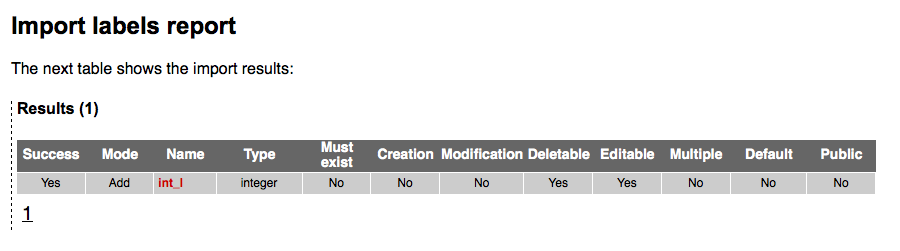
\includegraphics[scale=0.4]{import_labels.png}
  \caption{Import labels report}
  \label{fig:import_labels}
\end{figure}

The \textbf{Success} column tells if the label was successfully installed into the system
and the \textbf{Mode} column if the label is new to the system (mode \textit{add}) or the label
was already present and it was only updated (mode \textit{edit}).

\section{Sequences}

All sequence related options can be found in the \textbf{Sequences} submenu.
Three options can be found there: \textbf{List}, \textbf{Add/New} and \textbf{Batch}.

The \textbf{Sequences - List} option is used to list all system sequences. This page can also
be accessed without logging in, where only the labels annotated with the label \textbf{perm\_public}
as true will appear. This page also features a filter form.

More options are available in that page, namely:

\begin{itemize}
  \item \textbf{Search}: launches a new search page with the sequences present in the grid.
  
  \item \textbf{Add new}: redirects to a new page, where one can insert a new sequence.
\end{itemize}

To insert a new sequence one can use the \textbf{Add new} button or the \textbf{Sequences - Add/New}
option from the main menu. In the new sequence page, three fields are available: \textbf{Name}, for the
sequence name; \textbf{Content}, for the sequence content and \textbf{Generate protein}, that when the
sequence being insert is a DNA sequence, a protein sequence will be generated from it and the two sequences
will be automatically linked using the \textbf{translated} label.

Once the sequence is inserted, the user will be redirected to the sequence page (Figure \ref{fig:view_sequence}).
In this page, basic information about the sequence is shown, namely its name, content,
a link to the translated sequence, and, in the case of
sub-sequences, a link to the original sequence. In this page it is also possible to export the sequence,
by pushing the \textbf{Export} button.

The \textbf{Delete} button prompts you to delete the sequence and the \textbf{View labels} button
redirects you the sequence's label page.

\begin{figure}[H]
  \centering
    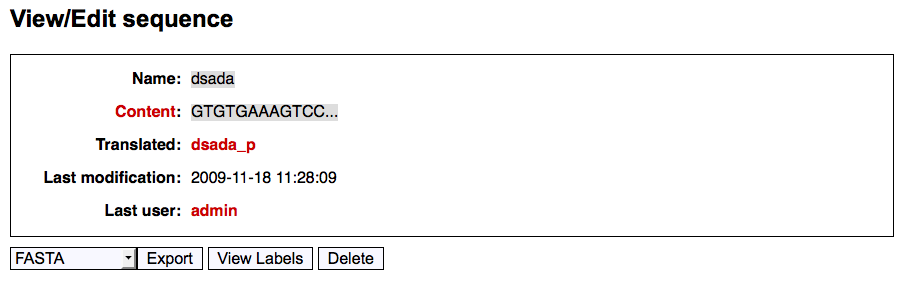
\includegraphics[scale=0.4]{view_sequence.png}
  \caption{Sequence page.}
  \label{fig:view_sequence}
\end{figure}

To edit sequence name or content just click in the respective name and content.

\subsection{Labels page}

Through the \textbf{View labels} button we can access the sequence's label page.

The labels page displays the sequence's annotated labels, labels available to add,
missing labels and non-multiple labels that have more than one instance for this sequence,
which we name the \textbf{bad multiple} labels.

The annotated labels list is always shown. The \textbf{Available} labels list
is only shown if the sequence is not annotated with every system label, which is the most frequent case.
The missing labels list is only shown if the sequence has not been annotated with
mandatory labels, like \textbf{type} or \textbf{length}. The bad multiple labels list
is only shown when, for some reason, the sequence is annotated with various instances of
the same label that is not multiple, this can happen when a label, once multiple, no longer is.

An example labels page in shown in Figure \ref{fig:labels2}. Some sets of labels are not shown
by default and must be displayed by clicking \textbf{Show}. Filtering of labels is also available
as shown in the example page.

\begin{figure}[ht]
  \centering
    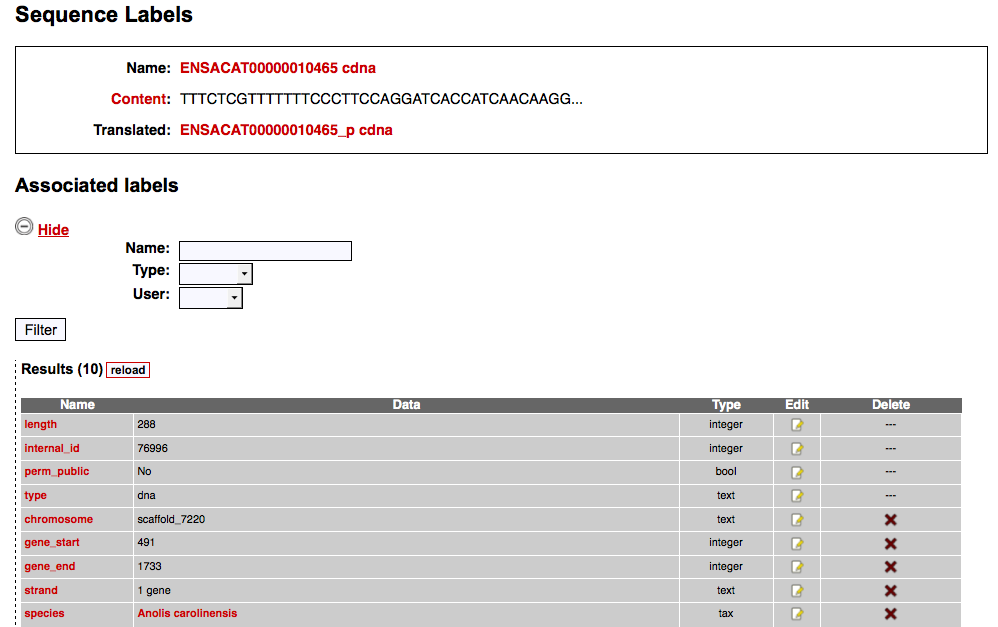
\includegraphics[scale=0.5]{labels.png}
  \caption{Example labels page.}
  \label{fig:labels2}
\end{figure}

Some useful interactions were implemented: clicking in one missing label opens the available pages
separator and highlights the label there, easing the process of annotating the sequence with missing
labels; clicking in one bad-multiple label highlights the specific label instance in the annotated labels list.

Clicking on the \textbf{Show details} link forces the annotated labels list to display more details
about the labels.

Multiple labels are shown as \textit{label\_name[parameter]}, where \textit{parameter} is the multiple
label parameter.

Clicking \textbf{Add} the icon from the first column of the \textbf{Available labels} list popups a new window
that will be used to create a new label instance. To delete any annotated label,
just use the icons from the \textbf{Delete} column
from the same list. The \textbf{Data} column displays the label value and for label types like
reference, object, taxonomy or URL, a link is rendered that redirects you to the resource.

The \textbf{Edit} icon from the annotated labels list
launches a new window to edit the current label value.
This window is similar to the one used to insert new label instances.

The edit or add label popup windows display forms where the user can insert or edit label values.

If the label supports automatic generation a checkbox \textbf{Generate default value} is displayed.
If checked in, the result will be a new label instance generated from the label code.

For each label type, the popup window is slightly different. Next's a summary is enumerated:

\begin{itemize}
  \item \textbf{integer}, \textbf{float}: text field with numeric validation.
  \item \textbf{text}: simple text field.
  \item \textbf{url}: text field with URL validation.
  \item \textbf{bool}: a checkbox.
  \item \textbf{position}: two text fields with numeric validation.
  \item \textbf{taxonomy}: a searchable grid with taxonomies that can be selected.
  \item \textbf{reference}: a searchable grid with sequences that can be selected.
  \item \textbf{date}: text field with calendar widget.
  \item \textbf{object} (Figure \ref{fig:obj_label2}): if the label has files attached a select list is displayed containing them.
  An upload field is also available.
\end{itemize}

\begin{figure}[ht]
  \centering
    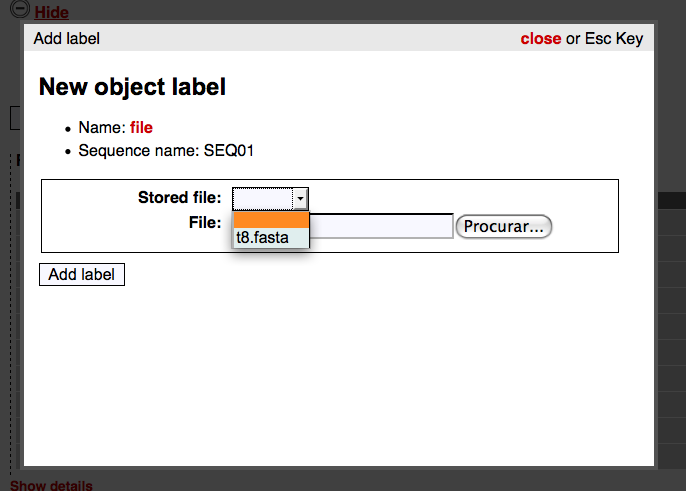
\includegraphics[scale=0.5]{obj_label.png}
  \caption{Annotating a new object label.}
  \label{fig:obj_label2}
\end{figure}

Once a label instance is added or edited the labels page is updated to reflect the changes.

\subsection{Batch}

Instead of inserting sequences one by one using the page described above, you can
upload a file with several sequences in either XML or FASTA format. These files
can be also annotated with labels as described in the section \ref{sec:file_formats}.

When uploading the file, the system will try to insert or update the stored sequences.
A sequence is only updated if the application can found a previously stored sequence with
the same name and content, everything else is treated as a new sequence.

To access this functionality use the \textbf{Sequences - Batch} main menu option.

In this page (Figure \ref{fig:sequence_upload2}) three options are available: upload a single file; upload both DNA and protein file, linking
the sequences along the process; upload a DNA file and also generate protein sequences.
When converting DNA to protein sequences, it is possible to annotate the protein sequences
with the same DNA labels by using the \textbf{Keep structure} option.

\begin{figure}[ht]
  \centering
    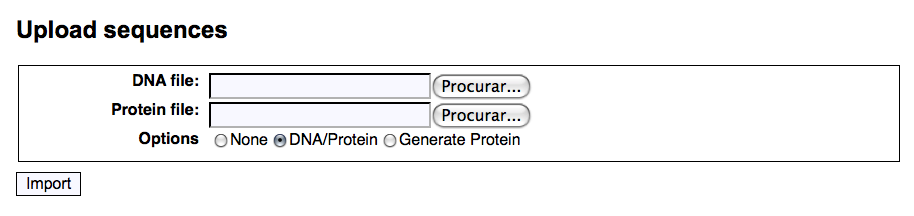
\includegraphics[scale=0.5]{sequence_upload.png}
  \caption{Upload sequences page.}
  \label{fig:sequence_upload2}
\end{figure}

When the file is being processed a loading screen appears displaying the progress.
When everything is done a report page like the Figure \ref{fig:batch_report2} should appear.

\begin{figure}[ht]
  \centering
    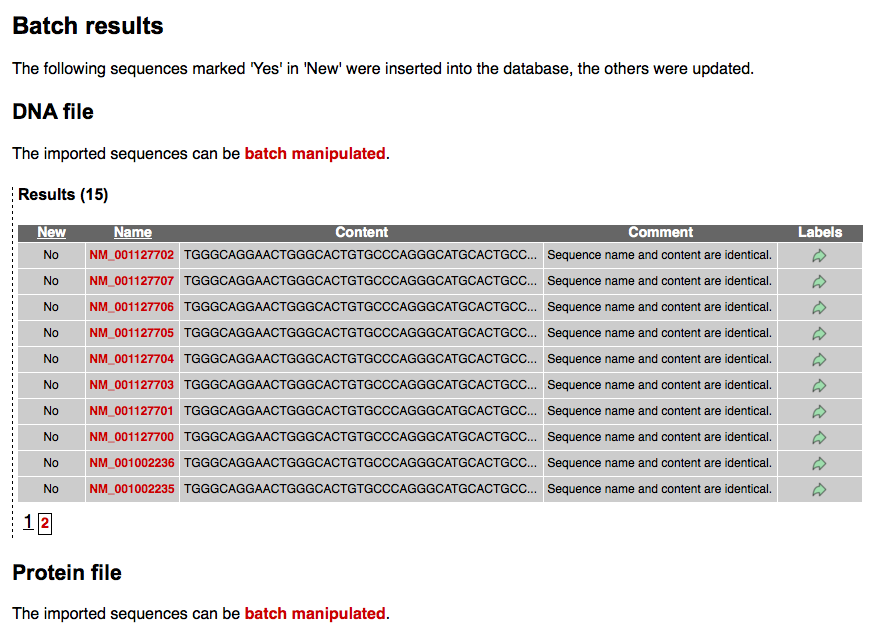
\includegraphics[scale=0.5]{batch_report2.png}
  \caption{Batch sequence report.}
  \label{fig:batch_report2}
\end{figure}

If the \textbf{none} option was chosen, only a list of sequences is shown, for everything else,
a list of DNA and protein sequences are shown.

If the files sent were annotated with labels, a label report is shown, indicating the state for each label.
For example, if a label present in the file is not installed in the system, a warning indicating the label
is not installed will be shown. Only previously installed labels will be used when importing label values.

In each sequence list the \textbf{New} column indicates if the sequence is new and was inserted, or if it is old
and it is being updated. The \textbf{Comment} label displays various kinds of informations and can tell when
the sequence was only updated.

If the file was annotated with labels, a column named \textbf{Status} will appear in the sequence list. Clicking
on the green arrow will popup a window with a grid, indicating for each label, the status for this sequence.
For example, if a label is automatically generated when a sequence is created and its value was specified in the file,
the label will not be updated and the text \textbf{Already inserted} will be shown.

Clicking on the \textbf{batch manipulated} link will redirect you to a new search page with only the imported sequences,
which is useful to run various operations for all those sequences in batch mode.

\section{Taxonomies}

To manage taxonomies we should pay attention to three things: trees, taxonomy ranks and taxonomies.

With taxonomy trees one can have multiple trees of taxonomies, which is useful to have custom
taxonomies and more scientific trees like the NCBI taxonomy tree.

Ranks is one way to categorize taxonomies. The system installs a rich set of ranks,
with parent/child relationships already defined.

To access taxonomy related features, use the \textbf{Taxonomies} submenu from the main menu.

\subsection{Managing trees}

To list the currently defined taxonomy trees, select \textbf{Taxonomies - Trees - List}, there
you should at least see the NCBI tree (Figure \ref{fig:tree_list}).

\begin{figure}[H]
  \centering
    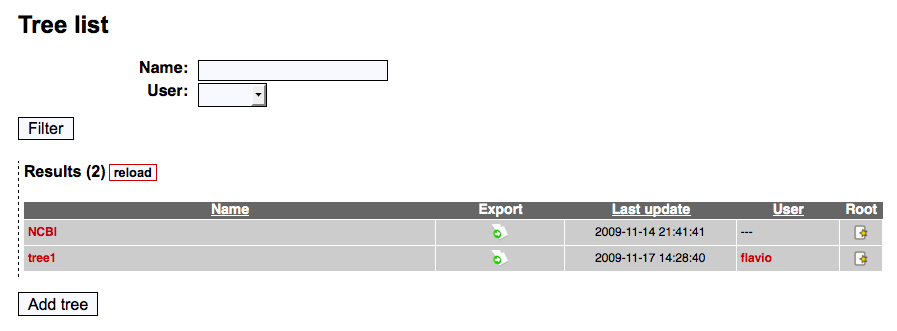
\includegraphics[scale=0.4]{tree_list.png}
  \caption{Tree listing.}
  \label{fig:tree_list}
\end{figure}

The user has the possibility to filter the tree list using a tree name or the user who made the last update.

From here you can select a tree to view or edit or select \textbf{Add tree} to create a new tree.
To create a new tree you can also use \textbf{Taxonomies - Trees - Add/New}.

Each tree can also be exported to a XML file using the green \textbf{Export} button.
The yellow \textbf{Root} button helps creating a new root taxonomy for this tree.

Selecting \textbf{Add tree}, you will be prompted for the tree name. Once created, you will be
redirected to the tree's page, as in Figure \ref{fig:view_tree}.

In it you can see history information and also edit the tree name by clicking on it.

There is also four operation buttons:

\begin{itemize}
  \item List trees: redirects you back to the tree list.
  \item Export: exports the tree to a XML file.
  \item Delete: prompts you to delete the tree (not available for the NCBI tree).
  \item Browse: enables you to browse the tree.
\end{itemize}

\begin{figure}[H]
  \centering
    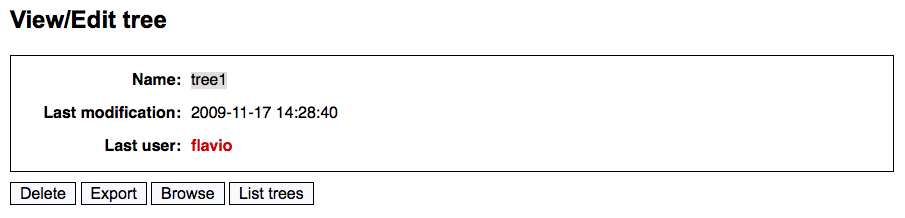
\includegraphics[scale=0.4]{view_tree.png}
  \caption{Viewing a tree.}
  \label{fig:view_tree}
\end{figure}

If you are an administrator you can make use of the option \textbf{Taxonomies - Trees - Import}
to upload a taxonomy tree XML file. Once the file is uploaded, the system tries to insert
all taxonomies from that tree into the system. If some taxonomies are found, updates are done.

\subsubsection{Tree browsing}

The tree browser page provides an easy to use interface to navigate through the target tree.

In Figure \ref{fig:tree_browsing} we are navigating the NCBI tree, currently at node \textbf{root}
and the grid is filled with \textbf{root}'s children.

We can go up in the hierarchy by clicking \textbf{Go up \textit{node name}}. To navigate into
a taxonomy we click the green arrow in the select column for that taxonomy. We can also
add a new taxonomy child, selecting the last icon from the \textbf{Child} column, it redirects us
to a new taxonomy form, with the parent taxonomy already setup.

\begin{figure}[H]
  \centering
    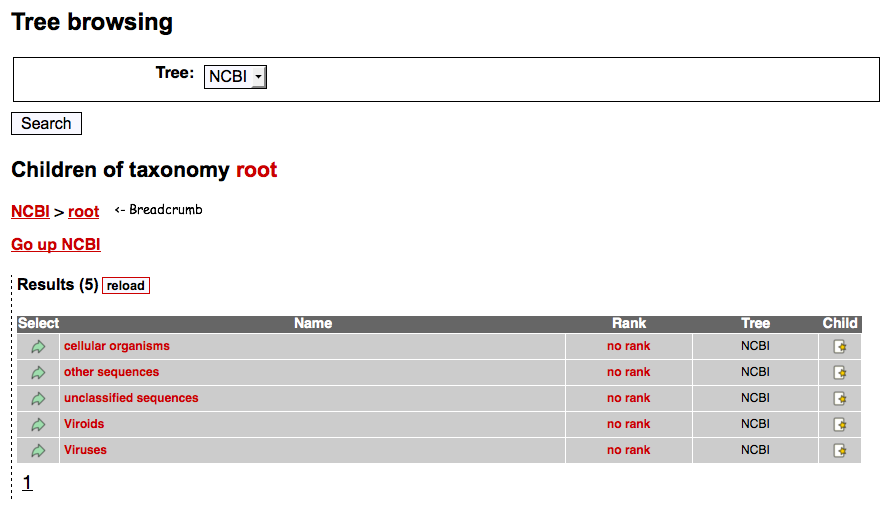
\includegraphics[scale=0.4]{tree_browsing.png}
  \caption{Browsing the NCBI tree.}
  \label{fig:tree_browsing}
\end{figure}

Another important aspect is the breadcrumb component (in the example \textbf{NCBI $>$ root}). Clicking
in one breadcrumb name will make the current taxonomy change.

\subsection{Managing ranks}

To list all system ranks use the option \textbf{Taxonomies - Ranks - List} from the main menu.
This page gives you a filter enabled rank list, being possible to filter the rank list by
rank name, parent rank name or the user who made the last rank change.

You can also order the rank names by alphabetical order, ascending or descending.

To export the current set of ranks just push the \textbf{Export all} button.

For each rank in the grid, there are two action icons: one named \textbf{Taxonomy}, that redirects us
to the new taxonomy form where the rank is already selected, and the other, \textbf{Child}
opens a new page with a form to create a new rank with the parent rank already set.

To create ranks, there's also the \textbf{Taxonomies - Ranks - Add/New} menu option.
On this page, you should input the rank name and select the parent rank from the list of inserted ranks.

Once a rank is created, the system redirects you to the rank page where you can edit the rank name
or parent rank by clicking in the respective name. Editing by clicking on the name, changes the rank name
to a text field, where you can input the new name and then, when pushing the \textbf{OK} button, sends the
changes back to the server.

Also, when on the rank page, there are two buttons at the end of the page: \textbf{Delete} prompts you to
delete the rank and \textbf{List ranks} redirects you back to the rank list.

\subsubsection{Import / Export}

When logged in as \textbf{admin} you can export all system ranks through the option
\textbf{Taxonomies - Ranks - Export}. The output file is XML.

The other way around, you can import a XML file with ranks, through the option
\textbf{Taxonomies - Ranks - Import}. Once the file is processed by the server
a page like Figure \ref{fig:rank_import} is shown.

The column \textbf{Success} tells if the new rank was installed into the system or not,
the column \textbf{Mode} indicates if the new rank was added or edited. The \textbf{Parent found}
column tells if the parent was found in the system (if the system can not find it, it is created).
The column \textbf{Original parent} was the rank parent before the import operation if the rank
was already in the system and the column \textbf{Parent} just indicates the new parent rank.

\begin{figure}[H]
  \centering
    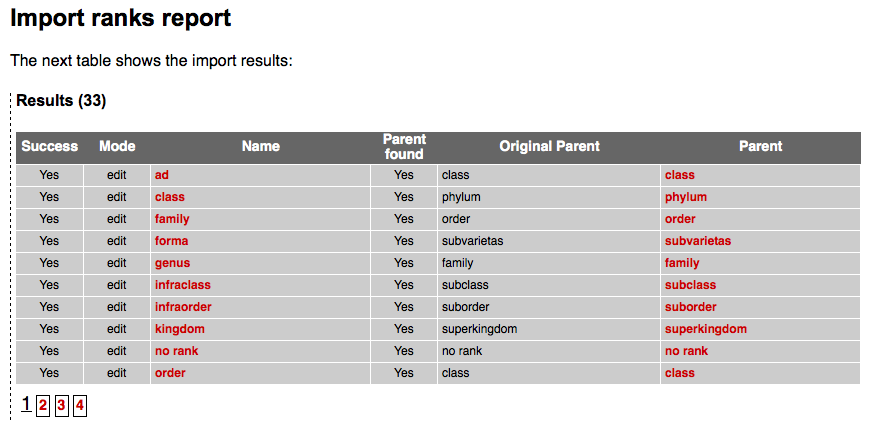
\includegraphics[scale=0.4]{rank_import.png}
  \caption{Import rank report}
  \label{fig:rank_import}
\end{figure}

\subsection{Managing taxonomies}

We have seen that there are lots of ways to get to the new taxonomy form. The standard way is to
choose the option \textbf{Taxonomies - Add/New} from the main menu. There you should enter the
taxonomy name, choose the rank and tree from a list of stored ranks and trees, respectively.

The rank and tree can be left empty, but as a recommendation, you should define them right
from the beginning.

Once a taxonomy is created, the system redirects you to the taxonomy page.
Each taxonomy page is composed of: a form where you can edit basic taxonomy information (Figure \ref{fig:taxonomy_basic}),
a list of optional taxonomy names (Figure \ref{fig:other_names}) and a list of children taxonomies.

In the first part (Figure \ref{fig:taxonomy_basic}), you can edit the name and rank by clicking in the respective name.
Changing the tree is not allowed. To change the parent you should click the red \textbf{Parent:} link and when
a window popup appears you should search for your parent taxonomy, select the name from the grid and then push
the \textbf{Select} button.

\begin{figure}[H]
  \centering
    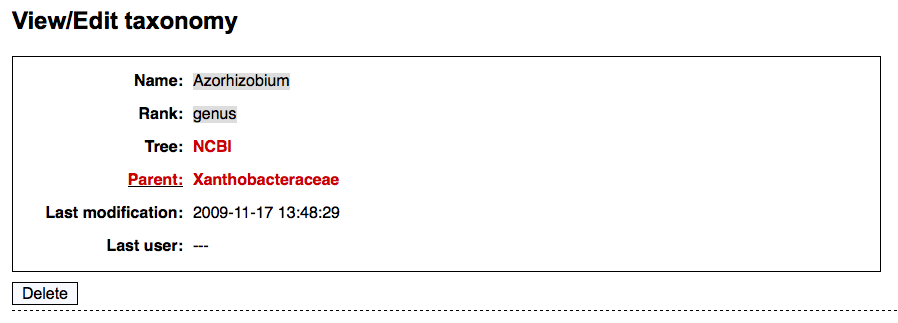
\includegraphics[scale=0.4]{taxonomy_basic.png}
  \caption{Editing taxonomy information.}
  \label{fig:taxonomy_basic}
\end{figure}

The \textbf{Other names} section provide a list of other names for the taxonomy. Each name can be deleted
using the \textbf{Delete} column. To edit a name you should click on the name cell and then push the \textbf{OK}
button. To edit the name type the process is identical. To add a name, just use the provided form.

\begin{figure}[H]
  \centering
    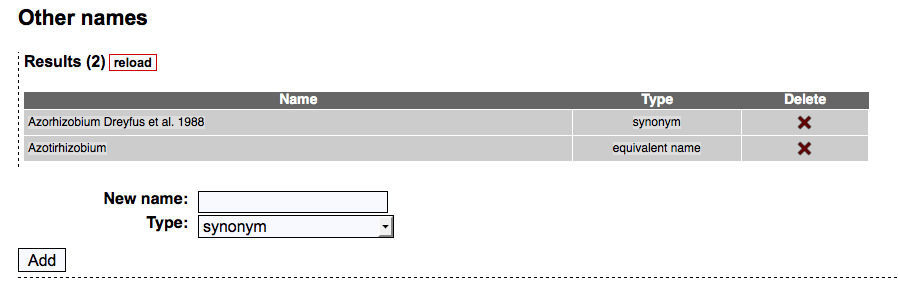
\includegraphics[scale=0.4]{other_names.png}
  \caption{Other names section.}
  \label{fig:other_names}
\end{figure}

The final section displays a grid with the children taxonomy. You can add new ones to the list by pushing
the \textbf{Add child} button.

As the number of taxonomies can get very large, we provided a page where one can search by taxonomies
by just using the name, tree or rank, or any combination of these.

To use this interface go to \textbf{Taxonomies - Browse}.

\section{Search}

To search sequences using the annotated label information, one can use the search pages available
from the main menu. Three pages are available:

\begin{itemize}
  \item \textbf{Search - ALL}: to search all sequences.
  \item \textbf{Search - DNA}: search only DNA sequences.
  \item \textbf{Search - Protein}: search only protein sequences.
\end{itemize}

All the three search pages look the same, so everything we will describe for the rest
of this section will apply for all of them.

Accessing any search page, we will rapidly discover three main sections in this page:
the query input section, the operations section and the preview section.

\subsection{Query input}

The query input section (as shown in Figure \ref{fig:search1_man}) presents you controls
to display and manipulate the query expression.

The query is presented in two formats: the tree, where you can manipulate parts of the expression
and the query text, where the query is presented in an human readable format. In the query tree view,
apart from selecting where to insert sub-expressions, you can also delete parts of the expression by
selecting an AND, OR, NOT or terminal expression and pressing \textbf{Delete}.

To insert a new query expression, you should choose where the expression will be put. That is possible
selecting one of the previously inserted OR, AND or NOT expressions. If you simply want
to create a simple AND query expression, press the \textbf{Reset} button and start
inserting expressions. But if you want to create complex queries you should know how to
insert expressions at different positions.

\begin{figure}[H]
  \centering
    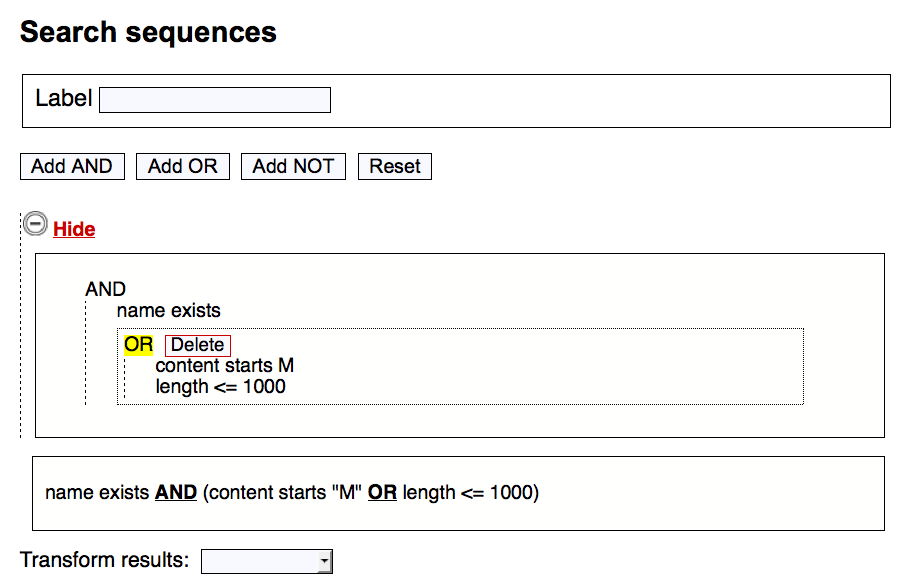
\includegraphics[scale=0.5]{search1.png}
  \caption{Search query input.}
  \label{fig:search1_man}
\end{figure}

When creating a new sub-expression, the process involves various steps:

\begin{itemize}
  \item First, input the label name you want to use for this term in the \textbf{Label} field.
  The system will autocomplete the label names as you type.
  \item When a label is chosen, you must select the search operator. Please see the table \ref{tbl:operators}
  for information about each operator.
  \item After the operator is chosen, you must, optionally, input the value for the operator.

  In resume, for each label type:
  
  \begin{itemize}
     \item Text, URL and Object: Text field.
     \item Integer, position and float: Numeric text field.
     \item Bool: Checkbox.
     \item Date: The date is input in a calendar widget. Please click on the text field to activate it.
     \item Taxonomy: Text field for the \textbf{like} operator. For the \textbf{equal} operator you should
      click on the \textbf{Find taxonomy} link, search a taxonomy within the popup window and then click on
      the chosen taxonomy name.
     \item Reference: Text field for the \textbf{like} operator. For the \textbf{equal} operator you should
      click on the \textbf{Find sequence} link, search a sequence within the popup window and then click on
      the chosen sequence.
  \end{itemize}

  \item Press the \textbf{Add term} button. The new term should appear on the query views, and the preview
  section will be automatically updated.
\end{itemize}

Please remember that you can use the \textbf{exists} and \textbf{not exists} operators. These
operators will filter sequences that are annotated with a label or not, respectively, and do not need
values.

If the label is multiple, you can, optionally, input the multiple parameter. If the multiple parameter is
not given, the search is done for all label instances. If given, the query will only use the specific label instance.

You can also insert AND, OR and NOT terms. Use the respective buttons.

\begin{table}[H]
  \scalebox{0.7}{%
    \begin{tabular}{ | c | p{1.2\textwidth} |}
      \hline
      \textbf{Label type} & \textbf{Operators} \\ \hline
      
      URL, text and object & \begin{itemize}
        \item equal: Equal comparison.
        \item contains: If the label contains a substring.
        \item starts: If the instance starts with.
        \item ends: Starts counterpart.
        \item regexp: Regular expression matching.
      \end{itemize} \\ \hline
      
      Bool & \begin{itemize}
        \item equal: Equal comparison.
      \end{itemize} \\ \hline
      
      Integer and float & \begin{itemize}
        \item $=$
        \item $>$
        \item $<$
        \item $>=$
        \item $<=$
      \end{itemize} \\ \hline
      
      Position & \begin{itemize}
        \item $=$
        \item $>$
        \item $<$
        \item $>=$
        \item $<=$
      \end{itemize} You should also select the position component, start or length for the term.
      \\ \hline
      
      Date & \begin{itemize}
        \item equal: Equal comparison.
        \item before: Date is before some date.
        \item after: Date is after some date.
      \end{itemize} \\ \hline
      
      Taxonomy & \begin{itemize}
        \item equal: Equal comparison.
        \item like: A taxonomy name to search for. Using this operator will make system search for all
        taxonomies in the database with this name and then the query will match if a sequence points to any of them.
      \end{itemize} \\ \hline
      
      Reference & \begin{itemize}
        \item equal: Equal comparison.
        \item like: A sequence name to search for. Works the same way as for taxonomies.
      \end{itemize} \\ \hline
  \end{tabular}}
  \caption{Label types and operators.}
  \label{tbl:operators}
\end{table}

One important option in this section is \textbf{Transform results}. Here you can select a reference label,
and the results will be transformed using the annotated reference label in each sequence.
If not all sequences are annotated with that label, the new result set will be smaller than the original.
If the reference label is multiple, the new result set can be potentially bigger.

Please note that the new, transformed, set will be used for the following operations.

\subsection{Operations}

While you create your complex query you can see the preview component getting refreshed,
with either the result total, or, optionally, the result list. Finally, once the query is built,
you can do operations on the results.

The operations section as it can be seen in Figure \ref{fig:search2_man}, contains various operations
you can do to the search result list.

\begin{figure}[H]
  \centering
    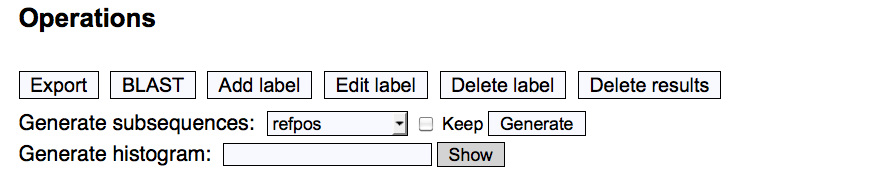
\includegraphics[scale=0.5]{search2.png}
  \caption{Search operations.}
  \label{fig:search2_man}
\end{figure}

\subsection{Sub-sequences}

We can generate sub-sequences using a position label from the result list. For example,
if your sequences contain a position label for a specific sequence segment, you can generate
sub-sequences for the complete set of sequences. To do that, you must select the position label
from the \textbf{Generate subsequences} select list and then push the \textbf{Generate button}.
If you want to keep your sub-sequences around longer than a few days, you should check the \textbf{Keep}
checkbox. When not keeping the sequences around, the system will delete them after some hours.

Once the sub-sequences are generated, a report page will be shown.

\subsection{BLAST}

The BLAST search option is used to do a BLAST search
over the result sequence list using an arbitrary number of 
query sequences.

The BLAST page is displayed on Figure \ref{fig:blast2} and shows two distinct
sections: section (1) for basic BLAST setup, section (2) for advanced parametrization.

\begin{figure}[ht]
  \centering
    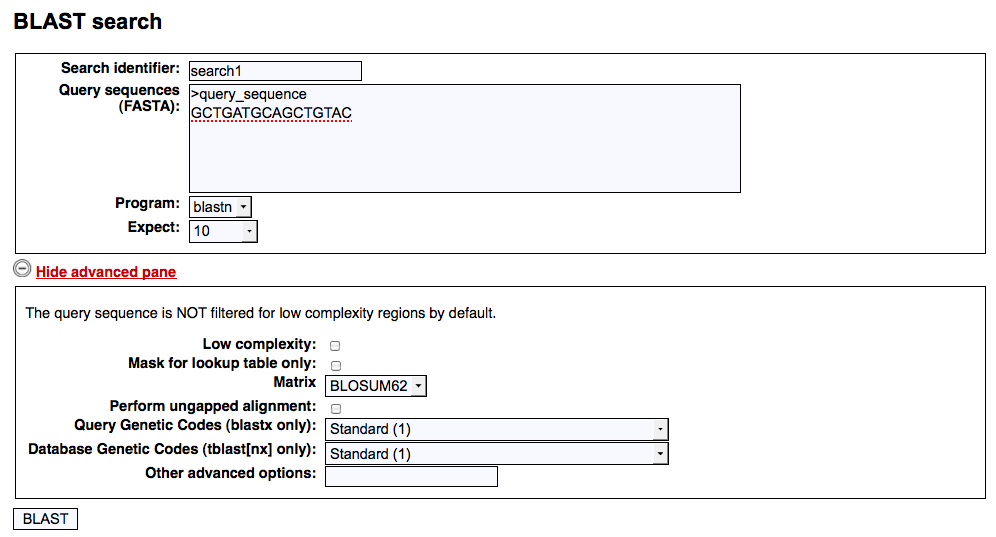
\includegraphics[scale=0.45]{blast.png}
  \caption{BLAST search screen.}
  \label{fig:blast2}
\end{figure}

In the first section, a search identifier must be provided, which identifies
this specific search and the query sequences in FASTA format that will be
matched against the result sequence list. It is also possible to
select between specialized BLAST programs, depending on the result sequence list
characteristics, but usually this option is pretty restricted by the system knowledge of
the sequences. Finally, the default \textit{expect} value can be changed to best
suit the search purposes.

The second section provides more advanced BLAST options.
If some BLAST option can not be found, the \textbf{Other advanced options} input box
is provided to pass arbitrary \texttt{blastall} program arguments.

Once the BLAST parameters are set, the \textbf{BLAST} button launches the BLAST
search and a new page is loaded (Figure \ref{fig:blast_results2}), presenting the BLAST output and a button to,
optionally, annotate each matched sequence with BLAST information.

\begin{figure}[ht]
  \centering
    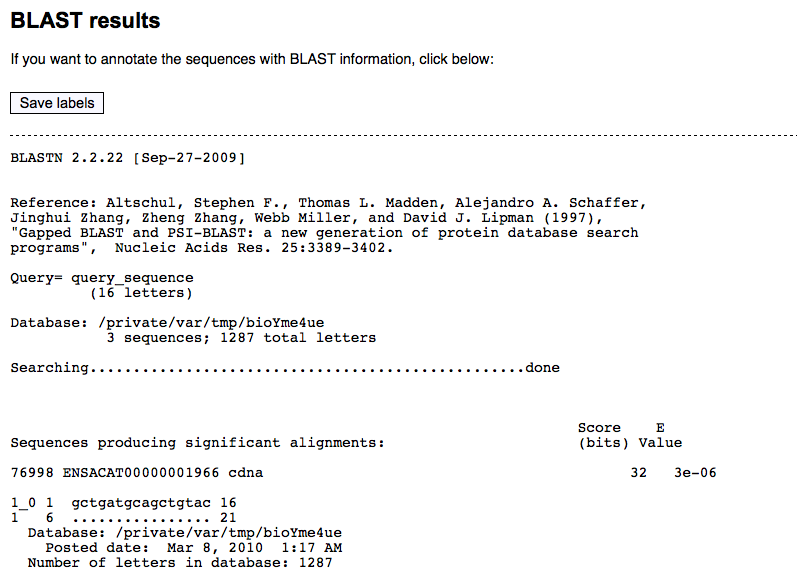
\includegraphics[scale=0.45]{blast_results.png}
  \caption{BLAST results screen.}
  \label{fig:blast_results2}
\end{figure}

The following labels are used:

\begin{itemize}
  \item \textbf{evalue} (float): Expectation value.
  \item \textbf{blast\_score} (float): BLAST score.
  \item \textbf{blast\_query} (boolean): True if the sequence matched the BLAST search.
\end{itemize}

Each one of these labels can have multiple instances and is parametrized by a search identifier
and the name of the matched query sequence.

For example, the search identifier provided was \textit{search1}, the
query sequences only included one sequence named \textit{query\_sequence} and
one sequence on the result list matched the query sequence.
The following annotations would be made:

\begin{itemize}
  \item \texttt{evalue[search1:query\_sequence] = 3e-06}
  \item \texttt{blast\_score[search1:query\_sequence] = 32}
  \item \texttt{blast\_query[search1:query\_sequence] = Yes}
\end{itemize}

\subsection{Histograms}

Another operation is the \textbf{Generate histogram} (Figure \ref{fig:histogram_man}).
This option can generate an histogram
for that label distribution across the result list. For example, you could generate a length
distribution for a given sequence set and then the system will generate the frequency histogram
and display the distribution total and number of classes.
For numeric labels the smallest class, largest class, average, median and mode values are also shown.

If your label is multiple and numeric, you can chose what value will be representative for each sequence.
You can use the average value for all label instances from a sequence, the minimum or the maximum value.
If the label is not numeric but multiple, all values will be considered.

\begin{figure}[ht]
  \centering
    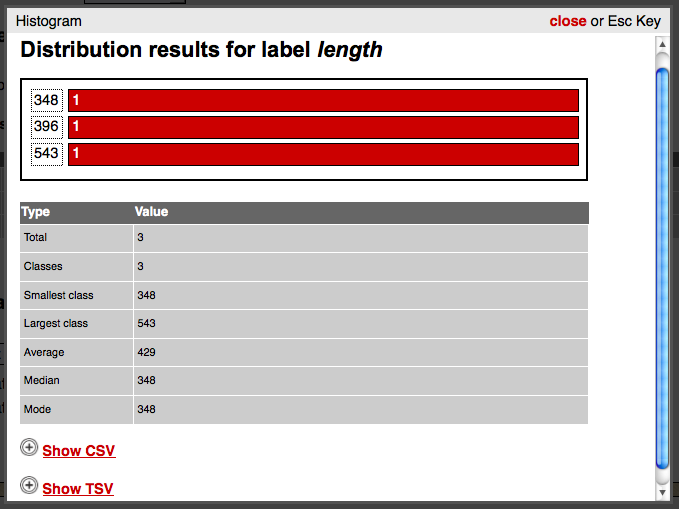
\includegraphics[scale=0.4]{histogram.png}
  \caption{Plotting histograms.}
  \label{fig:histogram_man}
\end{figure}

In the popup window that appears when generating the histogram, you can also copy the distribution values
to use with programs like Microsoft Excel.

\subsection{Export}

Another important operation is the \textbf{Export} button.
It can export your result sequences (Figure \ref{fig:export_search})
into the file formats mentioned before and supported by the system.

For formats like FASTA, CSV or XML, you can select the labels that will appear on the file, only exporting annotation 
that is important to the task at hand.

\begin{figure}[ht]
  \centering
    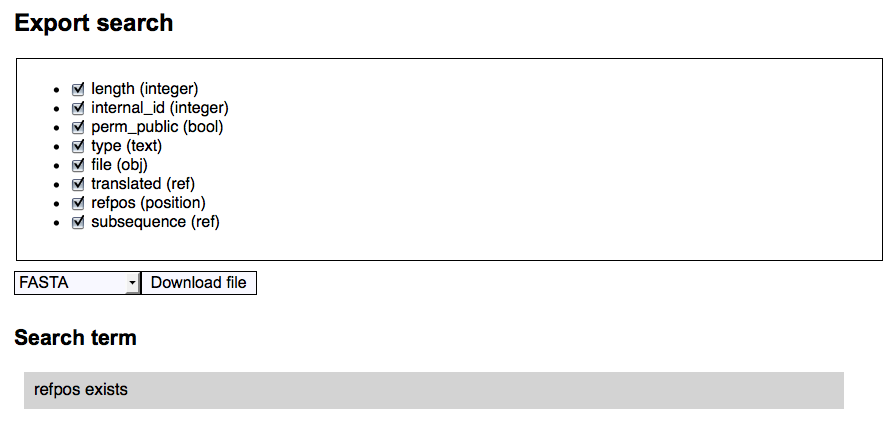
\includegraphics[scale=0.4]{export_search.png}
  \caption{Export search page.}
  \label{fig:export_search}
\end{figure}

\subsection{Batch labels}

Another common action to do is, for example, annotate a list of sequences with the same label instance.
For this you can use the button \textbf{Add label}, to add, or the button \textbf{Edit label}, to edit.

Using the \textbf{Add label} option you will be redirected to a page that looks like Figure \ref{fig:add_label_batch}.
First you should enter the label name into the \textbf{Label} text field, optionally you can check the \textbf{Update}
checkbox. When checked and if the sequence already contains that label instance, the current value will updated; if not
checked, nothing will be done.

When ready press the \textbf{Next...} button. A popup window should appear.
This window is very similar to the one we used to add a label to a sequence, so, it works the same way.

Once you input the label value, a report on the process should appear, right below the \textbf{Next...} button.

\begin{figure}[ht]
  \centering
    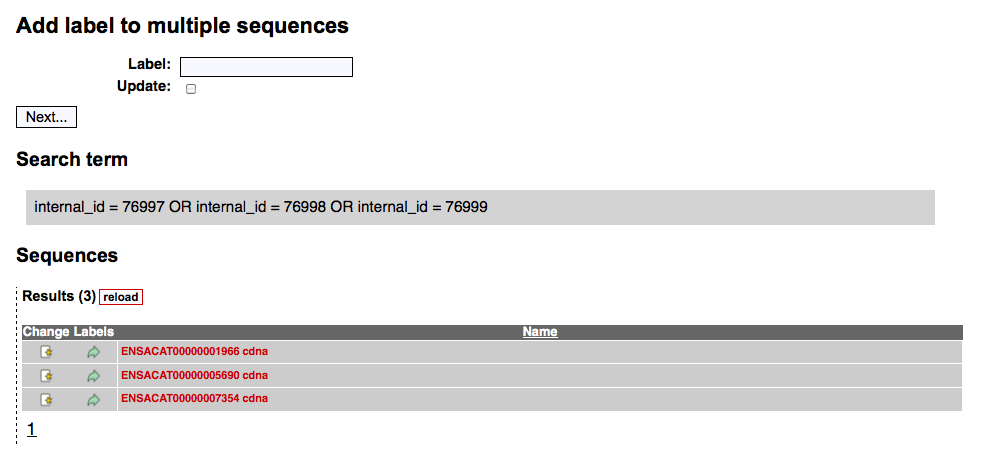
\includegraphics[scale=0.4]{add_label_batch.png}
  \caption{Add label to multiple sequences.}
  \label{fig:add_label_batch}
\end{figure}

The \textbf{Edit label} operation works in a similar fashion, but instead of having the \textbf{Update} checkbox,
it contains the \textbf{Add new} checkbox. This checkbox, when checked and when the sequence does not contain the
label, forces the system to add a new label value. It is the counterpart of the \textbf{Update} option, but for
the designed for the edit mode.

There is still another button, the \textbf{Delete label} button. This button gives you the possibility
to delete a label from the set of sequences. After you put the label, press the \textbf{Next...} button and
answer \textbf{Yes} and all annotations related to that label will disappear from the sequence list.

\subsection{Delete}

If you want to delete your sequence list just select the button \textbf{Delete} and
everything will be deleted. The action is irreversible, so use it with care!

\subsection{Preview}

The middle section (Figure \ref{fig:search3_man}) present in the search page is the preview section. In it
we can see the results for the query being build, as either the final total or the result list in a data grid.

\begin{figure}[H]
  \centering
    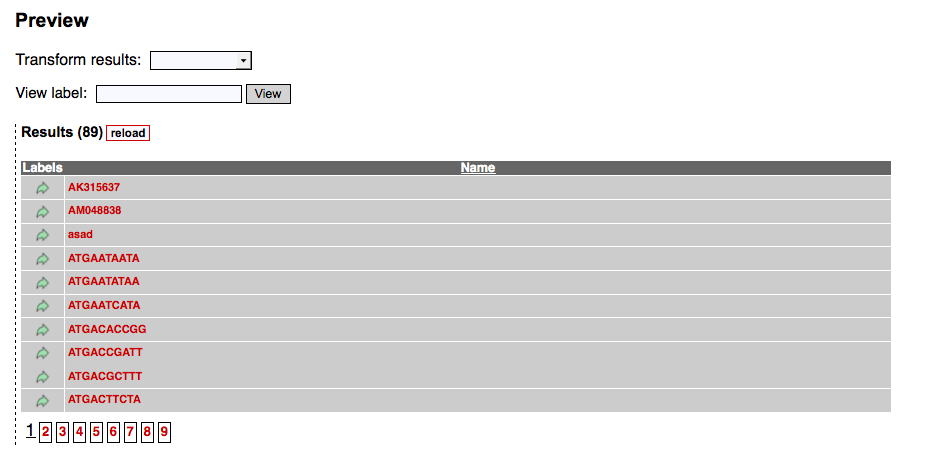
\includegraphics[scale=0.5]{search3.png}
  \caption{Search preview results.}
  \label{fig:search3_man}
\end{figure}

The \textbf{View label} option, can add new label columns to the result grid, showing the label
values for each sequence, as shown in Figure \ref{fig:view_label}.

\begin{figure}[H]
  \centering
    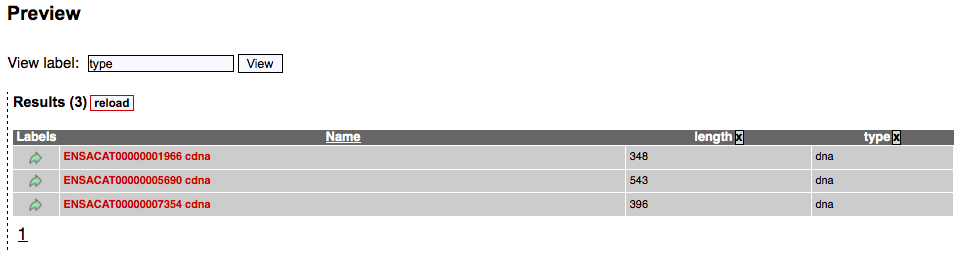
\includegraphics[scale=0.5]{view_label.png}
  \caption{Using view label.}
  \label{fig:view_label}
\end{figure}

Each new label column added can be removed by clicking the \textbf{X} on the column header.

\subsection{Written queries}

Instead of using the query input section from the search page, you can use the search field
on the top of each page to input arbitrarily complex queries.

The search field can also search for anything in the system: labels, taxonomies, ranks and sequences.
When the specified search expression is not valid, the system will fallback to a wide search for the
former objects, displaying a page with a grid for each entity where the query matched. So, for example,
if you input 'homo sapiens', the system will display a grid with taxonomies with 'homo sapiens' in the name.

But the more interesting case is when using valid query expressions. A query expression
is composed of terminal expressions and composed expressions.

A terminal expression contains a label name, an operator and, optionally, a value.
The following expression is a terminal expression: \textit{length $>$ 500}. The operators that
do not need a value, are the \textbf{exists} and \textbf{notexists} operators, like \textit{species exists}.
For everything else the form is \textit{label\_name operator value}. Operators and value information
is shown in table \ref{tbl:operators_values_expressions}.

Another note: if you want to write values with spaces, wrap the value around ' or ".

\begin{table}[ht]
  \scalebox{0.75}{%
    \begin{tabular}{ | c | p{0.4\textwidth} | p{0.7\textwidth} |}
      \hline
      \textbf{Label type} & \textbf{Operators} & \textbf{Values} \\ \hline
      
      URL, text and object & \begin{itemize}
        \item equal: Equal comparison.
        \item contains: If the label contains a substring.
        \item starts: If the instance starts with.
        \item ends: Starts counterpart.
        \item regexp: Regular expression matching.
      \end{itemize} & --- \\ \hline
      
      Bool & \begin{itemize}
        \item equal: Equal comparison.
      \end{itemize} & The value should be "true" or "false". \\ \hline
      
      Integer and float & \begin{itemize}
        \item $=$
        \item $>$
        \item $<$
        \item $>=$
        \item $<=$
      \end{itemize} & The value should be a number. \\ \hline
      
      Position & \begin{itemize}
        \item $=$
        \item $>$
        \item $<$
        \item $>=$
        \item $<=$
      \end{itemize} & Before the operator you should indicate the position component to compare: 'start' or 'length'. \\ \hline
      
      Date & \begin{itemize}
        \item equal: Equal comparison.
        \item before: Date is before some date.
        \item after: Date is after some date.
      \end{itemize} & Values should be in the form \textit{dd-mm-yyyy} like \textit{03-11-2009}. \\ \hline
      
      Taxonomy & \begin{itemize}
        \item like: A taxonomy name to search for.
      \end{itemize} & The \textbf{like} operator gets a taxonomy name and then searches all taxonomies
      with that name in the system and if the sequence points to any of them the query succeeds. \\ \hline
      
      Reference & \begin{itemize}
        \item like: A sequence name to search for.
      \end{itemize} & The values and operators work just like the taxonomy labels, but applied for sequences. \\ \hline
  \end{tabular}}
  \caption{Operators and values in query expressions.}
  \label{tbl:operators_values_expressions}
\end{table}

Now, composed expressions can combine various other expressions, recursively, and use the special operators: AND, OR or NOT.
AND and OR can be used like \textit{expression1 AND expression2 AND expression3 ...}. The NOT operator can only have
an expression as argument, like this: \textit{NOT expression}.

You can also use parenthesis to group expressions. So for example, you can have things like:
$<$\textit{(length $>$ 500 and name exists) or content regexp AGTG}$>$.

Once you input the expression, the system will analyze it and build a tree for it, redirecting you to the search page,
where you can run batch operations against the resulting sequences.

\section{File formats}

For file format information please read the section \ref{sec:file_formats} from the main technical report.

\section{Administration}

There are a few functionalities to do maintenance or administration tasks.
These tasks can only be used when logged in as \textbf{admin}.

\subsection{User management}

One of the key areas in administration is user management.
Lets see how we can add new users, update user settings and so forth.

\subsubsection{New user}

To create a new user select \textbf{Administration - Users - Register} and input the user information.
The username field is the name that should be used to login. You must also input the
user's password twice. Click \textbf{Do register}. If everything went well,
a new user has been registered and a list of all system users is shown.

This list can be accessed through \textbf{Administration - Users - List}.

Create more users as needed. You can also logout and try the new registered users if you want.

\subsubsection{User settings}

Given that only administrators can register new users, normal users can modify their information,
namely, the complete name, password, email and other settings.

To edit profile data, click on the user's name, below the main menu. The new page
presents user information and two buttons, as shown in Figure \ref{fig:settings}.

\begin{figure}[H]
  \centering
    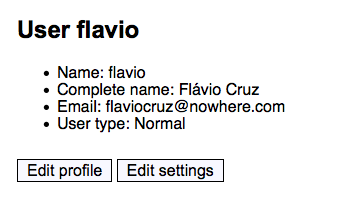
\includegraphics[scale=0.6]{settings.png}
  \caption{Page with user information.}
  \label{fig:settings}
\end{figure}

Selecting \textbf{Edit profile} enables us to edit the complete name, email or password.
When editing any information here, you should input your old password. If you want to change
the current password fill the two text fields for that, if not, leave them empty.

The other button, \textbf{Edit settings} enables you to change other, aspect related settings, like
the number of items per grid.

\subsubsection{Managing other users}

If you are an administrator using the \textbf{admin} account, you can edit other user profiles,
through \textbf{Administration - Users - List} and then selecting the target user. When editing
one user you should enter the \textbf{admin} password and not the user's current password.

For some reason, if you want to disable one user, go to the users list, select the user name
and click the \textbf{Delete} option.

One very destructive feature is the \textbf{Database reset}. It
can be accessed through the menu option \textbf{Administration - Reset Database} and removes all
custom data from the database, which is:

\begin{itemize}
  \item All taxonomy trees, except the NCBI tree.
  \item All ranks except the system defaults.
  \item All non-default labels.
  \item All sequences.
  \item All normal users.
  \item All files in the \textbf{file} table.
\end{itemize}

\subsection{Import / Export database}

Another useful feature is the database export / import facilities. One can
export the whole database as a XML file and then import it somewhere else, literally copying
the source database.

What is exported?

\begin{itemize}
  \item labels
  \item ranks
  \item taxonomy trees, except the NCBI tree
  \item sequences
\end{itemize}

To export the database, use the option \textbf{Administration - Export Database}.

To import a database XML file, go to \textbf{Administration - Import Database} from
the main menu. There you should upload the file and, once processed, an import report
is shown. The report is similar to the individual ones, but over various entities.

\subsection{Application customization}

There are two ways of customizing the application:

\begin{itemize}
  \item Changing the text that appears on the header: use the option \textbf{Administration - Database Description}.
  \item Changing the application's background: use the option \textbf{Administration - Database Background}. You should upload an JPG or PNG file.
\end{itemize}

\section{File formats} \label{sec:file_formats}


We use files to import or export data in order to interchange information between different kinds of systems or among various instances of the application. These files can be in two different kinds of formats: XML or FASTA.

Among other things, those files are used throughout the system to: copy entire databases, import sequences, install new labels, import whole taxonomy trees or heterogenous integration. 
 
\subsection{FASTA}

The FASTA format \cite{fasta} is very well known in the bioinformatics field as it is used to store a specific set of DNA or protein sequences.

In our system, this format is used to export stored sequences or to import new ones.

We have designed two FASTA-like formats:

\begin{itemize}
  \item Plain format
  
  In the plain format we just store the sequence name followed by its content.
  
\begin{lstlisting}[float, language=bash,frame=single,caption={Plain FASTA format.}]
>AK315637
ELRLRYCAPAGFALLKCNDADYDGFKTNCSNVSVVHCTNLMNTTVTTGLLLNGSYSENRT
QIWQKHRTSNDSALILLNKHYNLTVTCKRPGNKTVLPVTIMAGLVFHSQKYNLRLRQAWC
HFPSNWKGAWKEVKEEIVNLPKERYRGTNDPKRIFFQRQWGDPETANLWFNCHGEFFYCK
MDWFLNYLNNLTVDADHNECKNTSGTKSGNKRAPGPCVQRTYVACHIRSVIIWLETISKK
TYAPPREGHLECTSTVTGMTVELNYIPKNRTNVTLSPQIESIWAAELDRYKLVEITPIGF
APTEVRRYTGGHERQKRVPFVXXXXXXXXXXXXXXXXXXXXXXVQSQHLLAGILQQQKNL
LAAVEAQQQMLKLTIWGVK
<...more sequences...>
\end{lstlisting}
  
  \item Complex format
  
  In this format we also store label instance information along the sequence data. \\
  
  The format starts by including one line comment, followed by a line telling which labels are included for each sequence. Those labels are separated by the character '$|$'. If some label values are to be ignored, the label
  name should be skipped by placing an empty string followed by a '$|$'. \\
  
  For each sequence line we put all the label instances separated by the character '$|$'. The order of the label instances must be equal to the label's order at the file's header.\\
  
  If the sequence does not have a specific label instance the string in that column should be empty "".\\
  
  If the label instance value is empty and that label is not editable and can be generated from code it will be automatically generated when imported.
  
  For multiple labels, the label value is enclosed by square brackets '[]' and each instance, represented as \textit{param -$>$ value}, is separated by the character '§'.\\
  
  The special label 'name' is treated like any other label. If it is not included in the label's header, the
  first 10 sequence's content characters will be used by omission.
  
  An example of this format can be seen in Listing~\ref{ComplexFastaFormat}.\\
  
\begin{lstlisting}[float, language=bash,frame=single,breaklines=true,caption={Complex FASTA format example.}, label=ComplexFastaFormat]
;flavio - Monday 19th October 2009 07:06:33 PM - sequence id 465
#name|length|internal_id|perm_public|type|translated|url
>AK315637|1554|465|0|dna|AK315637_p|[google -> http://google.pt § ncbi -> http://www.ncbi.nlm.nih.gov/]
ELRLRYCAPAGFALLKCNDADYDGFKTNCSNVSVVHCTNLMNTTVTTGLLLNGSYSENRT
QIWQKHRTSNDSALILLNKHYNLTVTCKRPGNKTVLPVTIMAGLVFHSQKYNLRLRQAWC
HFPSNWKGAWKEVKEEIVNLPKERYRGTNDPKRIFFQRQWGDPETANLWFNCHGEFFYCK
MDWFLNYLNNLTVDADHNECKNTSGTKSGNKRAPGPCVQRTYVACHIRSVIIWLETISKK
TYAPPREGHLECTSTVTGMTVELNYIPKNRTNVTLSPQIESIWAAELDRYKLVEITPIGF
APTEVRRYTGGHERQKRVPFVXXXXXXXXXXXXXXXXXXXXXXVQSQHLLAGILQQQKNL
LAAVEAQQQMLKLTIWGVK (...)
<...more sequences...>
\end{lstlisting}
  
\end{itemize}

\subsection{XML}

The XML format is widely used to export and import lots of different kinds of data throughout the system. This format can handle labels, sequences, taxonomy trees, ranks and the database itself.

\begin{itemize}
  \item \textbf{Labels}
  
  Using the XML format we can export a set of labels. This file can then be imported in another system resulting in label installation or update. \\
  
  An example of this kind of file is shown in Listing~\ref{LabelXmlFile} and as it can be seen, we store each label property as a XML tag.
  
  All the rules concerning empty label instances from the complex FASTA format are also present in this format.
  
\begin{lstlisting}[float, language=xml, frame=single, label=LabelXmlFile, caption={An example Label XML file.}]
<labels>
  <label>
		<name>length</name>
		<type>integer</type>
		<comment></comment>
		<default>1</default>
		<must_exist>1</must_exist>
		<auto_on_creation>1</auto_on_creation>
		<auto_on_modification>1</auto_on_modification>
		<code>return strlen($content);</code>
		<valid_code>return $data &gt; 0;</valid_code>
		<editable>0</editable>
		<deletable>0</deletable>
		<multiple>0</multiple>
		<public>1</public>
	</label>
	<...more labels...>
</labels>
\end{lstlisting}

\item \textbf{Sequences}

Besides the FASTA format, sequences can also be stored in XML files. The main difference between the FASTA format is that, given the structured and flexible nature of XML, it is easier to describe the sequence contents and its label instances.

\begin{lstlisting}[float, language=xml, frame=single, label=SequenceXmlFile, caption={An Sequence XML file.}]
<sequences>
<author>flavio</author>
<date>Tuesday 20th October 2009 12:59:53 AM</date>
<what>sequence id 465</what>
<labels>
	<label>length</label>
	<label>internal_id</label>
	<label>perm_public</label>
	<label>type</label>
	<label>translated</label>
	<label>url</label>
</labels>
<sequence>
	<name>AK315637</name>
	<content>ELRLRYCAPAGFALLKCNDADYDGFKTNCSNVSVVHCTNLMNTTVTTGLLLNGSYSENRT
  QIWQKHRTSNDSALILLNKHYNLTVTCKRPGNKTVLPVTIMAGLVFHSQKYNLRLRQAWC
  HFPSNWKGAWKEVKEEIVNLPKERYRGTNDPKRIFFQRQWGDPETANLWFNCHGEFFYCK
  MDWFLNYLNNLTVDADHNECKNTSGTKSGNKRAPGPCVQRTYVACHIRSVIIWLETISKK
  TYAPPREGHLECTSTVTGMTVELNYIPKNRTNVTLSPQIESIWAAELDRYKLVEITPIGF
  APTEVRRYTGGHERQKRVPFVXXXXXXXXXXXXXXXXXXXXXXVQSQHLLAGILQQQKNL
  LAAVEAQQQMLKLTIWGVK (...)</content>
	<label name="length">1554</label>
	<label name="internal_id">465</label>
	<label name="perm_public">0</label>
	<label name="type">dna</label>
	<label name="translated">AK315637_p</label>
	<label name="url" param="google">http://google.pt</label>
	<label name="url" param="ncbi">http://www.ncbi.nlm.nih.gov/</label>
</sequence>
</sequences>
\end{lstlisting}

The same sequence represented in FASTA (Listing~\ref{ComplexFastaFormat}) can be seen formatted as XML in Listing~\ref{SequenceXmlFile}.
  
  \item \textbf{Ranks}
  
  To manage ranks across multiple application instances we designed a XML format to store taxonomy ranks.
  
\begin{lstlisting}[float, language=xml, frame=single, label=RankXmlFile, caption={An example Rank XML file.}]
<ranks>
	<rank>
		<name>class</name>
		<parent>phylum</parent>
	</rank>
	<rank>
		<name>family</name>
		<parent>order</parent>
	</rank>
	<...more ranks...>
</ranks>
\end{lstlisting}
  
  As it can be seen in Listing~\ref{RankXmlFile}, for each rank we register its name and parent rank. This type of files is useful to copy rank sets around systems.
  
  \item \textbf{Taxonomy trees}
  
  We designed a XML format to store taxonomy trees, which is very useful to easily copy an entire taxonomy tree from one system to another.
  
\begin{lstlisting}[float, language=xml, frame=single, label=TaxonomyTreeXmlFile, caption={An example Taxonomy tree XML file.}]
<tree>
	<name>example</name>
	<nodes>
		<taxonomy>
			<name>root_taxonomy</name>
			<rank>family</rank>
			<taxonomy>
				<name>child_taxonomy</name>
				<rank>genus</rank>
			</taxonomy>
			<taxonomy>
				<name>child_taxonomy2</name>
				<rank>genus</rank>
			</taxonomy>
		</taxonomy>
	</nodes>
</tree>
\end{lstlisting}
  
  In this format, we store the tree name followed by a 'nodes' tag which will store, starting by the root taxonomies, the taxonomies from this tree. Each 'taxonomy' tag may contain an arbitrary number of 'taxonomy' tags which represent taxonomy's children.
  
  \item \textbf{Database}
  
  We designed another XML based format, this time to store the entire database. The skeleton for this format is presented in Listing~\ref{DatabaseXmlFile} and it is organized as follows:
  
  \begin{itemize}
    \item \textbf{labels}
    
    This section is exactly the same as the Label XML file.
    
    \item \textbf{ranks}
    
    Idem, but for ranks.
    
    \item \textbf{trees}
    
    A special tag containing all the taxonomy trees. Each tree is represented the way it is shown for the Taxonomy tree XML file.
    
    \item \textbf{sequences}
    
    This section follows the Sequence XML file structure.
    
  \end{itemize}

  \begin{lstlisting}[float, language=xml, frame=single, label=DatabaseXmlFile, caption={Database in XML skeleton.}]
  <biodata>
    <...labels...>
    <...ranks...>
    <trees>
      <...all taxonomy trees...>
    </trees>
    <...sequences...>
  </biodata>
  \end{lstlisting}

\end{itemize}

\subsection{CSV}

The CSV format is used to display distribution values over a set
of sequences and a numeric label. Once copied, this information can be used in spreadsheet programs.

Another use of the CSV format is to export a sequence list and a selected set of labels.
The file header contains the list of labels that are represented and each line contains a single
sequence. Multiple label values are separated by the character \texttt{;} and each value is of
the form \texttt{paramater : value}.

An example CSV file is shown in Listing \ref{SequencesCSV}.

\begin{lstlisting}[float, language=bash, frame=single, label=SequencesCSV, caption={An example CSV file.}]
name , length , type
seq1 , 513 , dna
seq2 , 231 , protein
seq3 , 85 , dna
\end{lstlisting}
\section{Query language}\label{sec:grammar}

A simple, yet arbitrarily complex, query language was designed to search
stored sequences using annotated information present in label instances.

A simplified grammar in BNF format for this language is shown in Figure \ref{fig:query_bnf}.
Note that every label supports two basic unary operators: \textbf{exists} and \textbf{notexists}, when
used they filter sequences that contain any value label or no value at all, respectively.
Queries can be nested using the AND, OR and NOT operators. Parenthesis can also be used to group expressions.

\begin{figure}[ht]
\begin{grammar} 
[(colon){$\rightarrow$}] 
[(semicolon)$|$] 
[(comma){}] 
[(period){\\}] 
[(quote){\begin{bf}}{\end{bf}}] 
[(nonterminal){$\langle$}{$\rangle$}]
<expression>:<expression> AND <expression>; <expression> OR <expression>; NOT <expression>;(<expression>) ; <terminal>.
<terminal>:<label name>,<unary operators>;<bool terminal>;<integer terminal>;<float terminal>;<position terminal>;<taxonomy terminal>;<text terminal>;<url terminal>; <obj terminal>; <date terminal>.
<bool terminal>:<label name>;<label name>,<bool operators>,<bool value>.
<bool operators>:<base operators>.
<bool value>: "true"; "false".
<unary operators>:"exists";"notexists".
<base operators>:"is"; "$=$"; "eq"; "equal".
<integer terminal>:<label name>,<numeric operators>,<integer value>.
<float terminal>:<label name>,<numeric operators>,<float value>.
<position terminal>:<label name>,<position type>,<numeric operators>,<integer value>.
<numeric operators>:<base operators>;"$\greaterthan$"; "$\greaterthan=$"; "$\lessthan$"; "$\lessthan=$".
<position type>:"start";"length".
<taxonomy terminal>:<label name>,<taxonomy operators>,<label value>.
<taxonomy operators>:<base operators>; "like".
<url terminal>:<label name>,<text operators>,<url>.
<text terminal>:<label name>,<text operators>,<label value>.
<text operators>:<base operators>;"contains"; "starts"; "ends"; "regexp".
<obj terminal>:<text terminal>.
<date terminal>:<label name>,<date operators>,<date value>.
<date operators>:<base operators>; "after"; "before".
<date value>:<day>,"-", <month>, "-", <year>.
<label name>: <base label name>;<base label name>, "[", <string>, "]".
<base label name>:"{\tt\quotesymbol}",<string>,"{\tt\quotesymbol}"; <string>.
<label value>:"{\tt\quotesymbol}",<string>,"{\tt\quotesymbol}"; <string>.
\end{grammar}
\caption{Query language written in BNF.}
\label{fig:query_bnf}
\end{figure}

All labels support a basic set of operators: \textbf{is}, \textbf{=}, \textbf{eq} and \textbf{equal}. All those operators do the same thing and, depending on the label type, they filter sequences which contain the specified label value.

We can also specify a multiple label instance with the parameter selector, using \textit{label\_name{[parameter]}}. If an expression involves a multiple label that is not parameter specific, all label instances will be considered, instead of only one.

The following list specifies the differences for each label type:

\begin{itemize}
  \item \textbf{Bool}
  
  Labels of this type can use the equal operation on values \textit{true} or \textit{false}. We can also skip the operator and value altogether and only keep the label name, as the example: \textit{dna and length $>$ 5} instead of \textit{dna is true and length $>$ 5}. 
  
  \item \textbf{Integer and float}
  
  Numeric labels use the basic comparison operators: \textbf{=}, \textbf{$>$}, \textbf{$>=$}, \textbf{$<$}, \textbf{$<=$}.

  \item \textbf{Position}
  
  For position labels we must first select between the start or the length component, and then an integer operator.
  Example: \textit{label\_name start $>$ 5}.
  
  \item \textbf{Taxonomy and reference}
  
  For these kinds of labels we can also use the operator \textbf{like}, which has the same effect as the standard equal operator. Those operators work by searching all sequences or taxonomies where the name matches the provided regular expression and then filtering the result list of sequences who have at least one label instance point to the same sequence or taxonomy of the former search result.
  
  \item \textbf{Url and text}
  
  For these label types the operators provided are: \textbf{starts} (if the string starts with the provided value),
  \textbf{ends} and \textbf{regexp}, for regular expression matches.
  
  \item \textbf{Object}
  
  Object labels can use the same text operators to search the filename associated with the label instance.
  
  \item \textbf{Date}
  
  Date labels provide day based operators: \textbf{equal} (in the same day), \textbf{after} (after the day),
  \textbf{before} (before the day).
\end{itemize}

\clearpage
\renewcommand{\bibname}{References} 
\begin{thebibliography}
  {10}
  \bibitem{php} PHP: HyperText Preprocessor, \url{http://www.php.net/}
	\bibitem{fasta} FASTA format description, \url{http://www.ncbi.nlm.nih.gov/blast/fasta.shtml}
	  
\end{thebibliography}

\end{document}
